\documentclass[11pt]{article}
\usepackage{amsmath,amssymb,amsmath,amsthm,amsfonts}
\usepackage{latexsym,graphicx}
\usepackage{fullpage,color}
\usepackage{url}
\usepackage[pdftex,bookmarks,colorlinks=true,citecolor=blue]{hyperref}
\usepackage[numbers]{natbib}
\usepackage{graphicx,subfigure}
\usepackage{algorithm}
\usepackage{algorithmic}
\usepackage{listings}
\usepackage{xcolor}
\usepackage{color}

\numberwithin{equation}{section}

\pagestyle{plain}

\setlength{\oddsidemargin}{0in}
\setlength{\topmargin}{0in}
\setlength{\textwidth}{6.5in}
\setlength{\textheight}{8.5in}

\newtheorem{fact}{Fact}[section]
\newtheorem{question}{Question}[section]
\newtheorem{lemma}{Lemma}[section]
\newtheorem{theorem}[lemma]{Theorem}
\newtheorem{assumption}[lemma]{Assumption}
\newtheorem{corollary}[lemma]{Corollary}
\newtheorem{prop}[lemma]{Proposition}
\newtheorem{claim}{Claim}[section]
\newtheorem{remark}{Remark}[section]
\newtheorem{definition}{Definition}[section]
\newtheorem{prob}{Problem}[section]
\newtheorem{conjecture}{Conjecture}[section]
\newtheorem{property}{Property}[section]

\def\A{{\bf A}}
\def\a{{\bf a}}
\def\B{{\bf B}}
\def\bb{{\bf b}}
\def\C{{\bf C}}
\def\c{{\bf c}}
\def\D{{\bf D}}
\def\d{{\bf d}}
\def\E{{\bf E}}
\def\e{{\bf e}}
\def\F{{\bf F}}
\def\f{{\bf f}}
\def\g{{\bf g}}
\def\h{{\bf h}}
\def\G{{\bf G}}
\def\H{{\bf H}}
\def\I{{\bf I}}
\def\K{{\bf K}}
\def\k{{\bf k}}
\def\LL{{\bf L}}
\def\M{{\bf M}}
\def\m{{\bf m}}
\def\N{{\bf N}}
\def\n{{\bf n}}
\def\PP{{\bf P}}
\def\pp{{\bf p}}
\def\Q{{\bf Q}}
\def\q{{\bf q}}
\def\R{{\bf R}}
\def\rr{{\bf r}}
\def\S{{\bf S}}
\def\s{{\bf s}}
\def\T{{\bf T}}
\def\tt{{\bf t}}
\def\U{{\bf U}}
\def\u{{\bf u}}
\def\V{{\bf V}}
\def\v{{\bf v}}
\def\W{{\bf W}}
\def\w{{\bf w}}
\def\X{{\bf X}}
\def\x{{\bf x}}
\def\Y{{\bf Y}}
\def\y{{\bf y}}
\def\Z{{\bf Z}}
\def\z{{\bf z}}
\def\0{{\bf 0}}
\def\1{{\bf 1}}



\def\AM{{\mathcal A}}
\def\CM{{\mathcal C}}
\def\DM{{\mathcal D}}
\def\EM{{\mathcal E}}
\def\GM{{\mathcal G}}
\def\FM{{\mathcal F}}
\def\IM{{\mathcal I}}
\def\JM{{\mathcal J}}
\def\KM{{\mathcal K}}
\def\LM{{\mathcal L}}
\def\NM{{\mathcal N}}
\def\OM{{\mathcal O}}
\def\PM{{\mathcal P}}
\def\SM{{\mathcal S}}
\def\TM{{\mathcal T}}
\def\UM{{\mathcal U}}
\def\VM{{\mathcal V}}
\def\WM{{\mathcal W}}
\def\XM{{\mathcal X}}
\def\YM{{\mathcal Y}}
\def\RB{{\mathbb R}}
\def\RBmn{{\RB^{m\times n}}}
\def\EB{{\mathbb E}}
\def\PB{{\mathbb P}}

\def\TX{\tilde{\bf X}}
\def\TA{\tilde{\bf A}}
\def\tx{\tilde{\bf x}}
\def\ty{\tilde{\bf y}}
\def\TZ{\tilde{\bf Z}}
\def\tz{\tilde{\bf z}}
\def\hd{\hat{d}}
\def\HD{\hat{\bf D}}
\def\hx{\hat{\bf x}}
\def\nysA{{\tilde{\A}_c^{\textrm{nys}}}}

\def\alp{\mbox{\boldmath$\alpha$\unboldmath}}
\def\bet{\mbox{\boldmath$\beta$\unboldmath}}
\def\epsi{\mbox{\boldmath$\epsilon$\unboldmath}}
\def\etab{\mbox{\boldmath$\eta$\unboldmath}}
\def\ph{\mbox{\boldmath$\phi$\unboldmath}}
\def\pii{\mbox{\boldmath$\pi$\unboldmath}}
\def\Ph{\mbox{\boldmath$\Phi$\unboldmath}}
\def\Ps{\mbox{\boldmath$\Psi$\unboldmath}}
\def\ps{\mbox{\boldmath$\psi$\unboldmath}}
\def\tha{\mbox{\boldmath$\theta$\unboldmath}}
\def\Tha{\mbox{\boldmath$\Theta$\unboldmath}}
\def\muu{\mbox{\boldmath$\mu$\unboldmath}}
\def\Si{\mbox{\boldmath$\Sigma$\unboldmath}}
\def\si{\mbox{\boldmath$\sigma$\unboldmath}}
\def\Gam{\mbox{\boldmath$\Gamma$\unboldmath}}
\def\Lam{\mbox{\boldmath$\Lambda$\unboldmath}}
\def\De{\mbox{\boldmath$\Delta$\unboldmath}}
\def\de{\mbox{\boldmath$\delta$\unboldmath}}
\def\Ome{\mbox{\boldmath$\Omega$\unboldmath}}
\def\Pii{\mbox{\boldmath$\Pi$\unboldmath}}
\def\varepsi{\mbox{\boldmath$\varepsilon$\unboldmath}}
\newcommand{\ti}[1]{\tilde{#1}}
\def\Ncal{\mathcal{N}}
\def\argmax{\mathop{\rm argmax}}
\def\argmin{\mathop{\rm argmin}}

\def\ALG{{\AM_{\textrm{col}}}}

\def\mean{\mathsf{mean}}
\def\std{\mathsf{std}}
\def\bias{\mathsf{bias}}
\def\var{\mathsf{var}}
\def\sgn{\mathsf{sgn}}
\def\tr{\mathsf{tr}}
\def\rk{\mathrm{rank}}
\def\nnz{\mathsf{nnz}}
\def\poly{\mathrm{poly}}
\def\diag{\mathsf{diag}}
\def\Diag{\mathsf{Diag}}
\def\const{\mathrm{Const}}
\def\st{\mathsf{s.t.}}
\def\vect{\mathsf{vec}}
\def\sech{\mathrm{sech}}
\def\sigmoid{\mathsf{sigmoid}}

\newcommand{\red}[1]{{\color{red}#1}}



\def\argmax{\mathop{\rm argmax}}
\def\argmin{\mathop{\rm argmin}}

\newenvironment{note}[1]{\medskip\noindent \textbf{#1:}}%
        {\medskip}


\newcommand{\etal}{{\em et al.}\ }
\newcommand{\assign}{\leftarrow}
\newcommand{\eps}{\epsilon}

\newcommand{\opt}{\textrm{\sc OPT}}
\newcommand{\script}[1]{\mathcal{#1}}
\newcommand{\ceil}[1]{\lceil #1 \rceil}
\newcommand{\floor}[1]{\lfloor #1 \rfloor}



\lstset{ %
extendedchars=false,            % Shutdown no-ASCII compatible
language=Python,                % choose the language of the code
xleftmargin=1em,
xrightmargin=1em,
basicstyle=\footnotesize,    % the size of the fonts that are used for the code
tabsize=3,                            % sets default tabsize to 3 spaces
numbers=left,                   % where to put the line-numbers
numberstyle=\tiny,              % the size of the fonts that are used for the line-numbers
stepnumber=1,                   % the step between two line-numbers. If it's 1 each line
                                % will be numbered
numbersep=5pt,                  % how far the line-numbers are from the code   %
keywordstyle=\color[rgb]{0,0,1},                % keywords
commentstyle=\color[rgb]{0.133,0.545,0.133},    % comments
stringstyle=\color[rgb]{0.627,0.126,0.941},      % strings
backgroundcolor=\color{white}, % choose the background color. You must add \usepackage{color}
showspaces=false,               % show spaces adding particular underscores
showstringspaces=false,         % underline spaces within strings
showtabs=false,                 % show tabs within strings adding particular underscores
frame=single,                 % adds a frame around the code
%captionpos=b,                   % sets the caption-position to bottom
breaklines=true,                % sets automatic line breaking
breakatwhitespace=false,        % sets if automatic breaks should only happen at whitespace
%title=\lstname,                 % show the filename of files included with \lstinputlisting;
%                                % also try caption instead of title
mathescape=true,escapechar=?    % escape to latex with ?..?
escapeinside={\%*}{*)},         % if you want to add a comment within your code
%columns=fixed,                  % nice spacing
%morestring=[m]',                % strings
%morekeywords={%,...},%          % if you want to add more keywords to the set
%    break,case,catch,continue,elseif,else,end,for,function,global,%
%    if,otherwise,persistent,return,switch,try,while,...},%
}


\begin{document}

%\setlength{\fboxrule}{.5mm}\setlength{\fboxsep}{1.2mm}
%\newlength{\boxlength}\setlength{\boxlength}{\textwidth}
%\addtolength{\boxlength}{-4mm}


\title{Deep Reinforcement Learning}

\author{\textbf{Shusen Wang} \\ Stevens Institute of Technology}

%\date{ }

\maketitle

\begin{abstract}
This lecture note briefly summarizes three kinds of deep reinforcement learning approaches: value-based methods, policy-based methods, and actor-critic methods.
This note is structured as following.
First, reinforcement learning terminologies are defined.
Second, we study Deep Q Network (DQN), a family of value-based methods, and train DQN using temporal difference (TD) learning.
Third, we study policy-based learning and derive policy gradient algorithms.
Last, we study standard (random) actor-critic method and deterministic actor-critic method.
\end{abstract}



\section{Notation}

Throughout, we use uppercase letters, e.g., $X$, to denote random variables and lowercase letters, e.g., $x$, to denote their observations.
Let $\PB (X = x)$ be the probability of the event ``$X = x$''.
Let $\PB (Y=y | X=x)$ be the probability of the event ``$Y=y$'' under the condition ``$X=x$''.

\paragraph{Agent:}
A system that is embedded in an environment and takes actions to change the state of the environment. Examples include robots, industrial controllers, and Mario in the game Super Mario.


\paragraph{State ($S$):}
State can be viewed as a summary of the history of the system that determines its future evolution.
State space $\SM$ is the set that contains all the possible states.
At time step $t$, the past states are observed and we thus know their values: $s_1, \cdots , s_t$;
however, the future states $S_{t+1}, S_{t+2}, \cdots $ are unobserved random variables.


\paragraph{Action ($A$):}
The agent's decision based on the state and other considerations.
Action space $\AM$ is the set that contains all the actions.
Action space can be a discrete set such as $\{\textrm{``left''}, \textrm{``right''}, \textrm{``up''} \}$ or a continuous set such as $[0, 1] \times [-90, 90]$.
At time step $t$, the past actions are observed: $a_1, \cdots , a_t$, but the future actions $A_{t+1}, A_{t+2}, \cdots$ are unobserved random variables.


\paragraph{Reward ($R$):}
Reward is a value received by the agent from the environment as a direct response to the agent’s actions.
At time step $t$, all the past rewards are observed: $r_1, r_2, \cdots , r_t$.
However, the future reward $R_i$ (for $i > t$) is unobserved, and it depends on the random variables, $S_{t+1}$ and $A_{t+1}$.
Thus, at time step $t$, the future rewards $R_{t+1}, R_{t+2} , \cdots$ are random variables.




\paragraph{Policy function ($\pi $):}
The decision-making function of the agent. 
Policy is the probability density function (PDF): $\pi (a | s) = \PB ( A = a | S  = s )$.
The policy function maps the observed state $S=s$ to a probability distribution over all the actions in set $\AM$.
Since $\pi$ is a PDF, $\sum_{a \in \AM } \pi (a | s) = 1$.
The agent will perform action $a$ with probability $\pi (a | s)$, for all $a \in \AM$.
See the illustration in Figure~\ref{fig:random}.



\paragraph{State transition ($p $):}
Given the current state $S=s$, the agent's action $A=a$ will lead to the new state $S'$ given by the environment.
State-transition function is the probability density function (PDF) $p (s' | s, a) = \PB ( S'  = s' | S = s , A = a )$.
The environment makes $s'$ the new state with probability $p (s' | s, a)$, for all $s' \in \SM$.






\paragraph{Trajectory:}
The agent's interaction with the environment results in a sequence of (state, action, reward) triplets:
$s_1, a_1, r_1, s_2, a_2, r_2, s_3, a_3, r_3, \cdots$

\begin{figure}[!t]
    \centering
    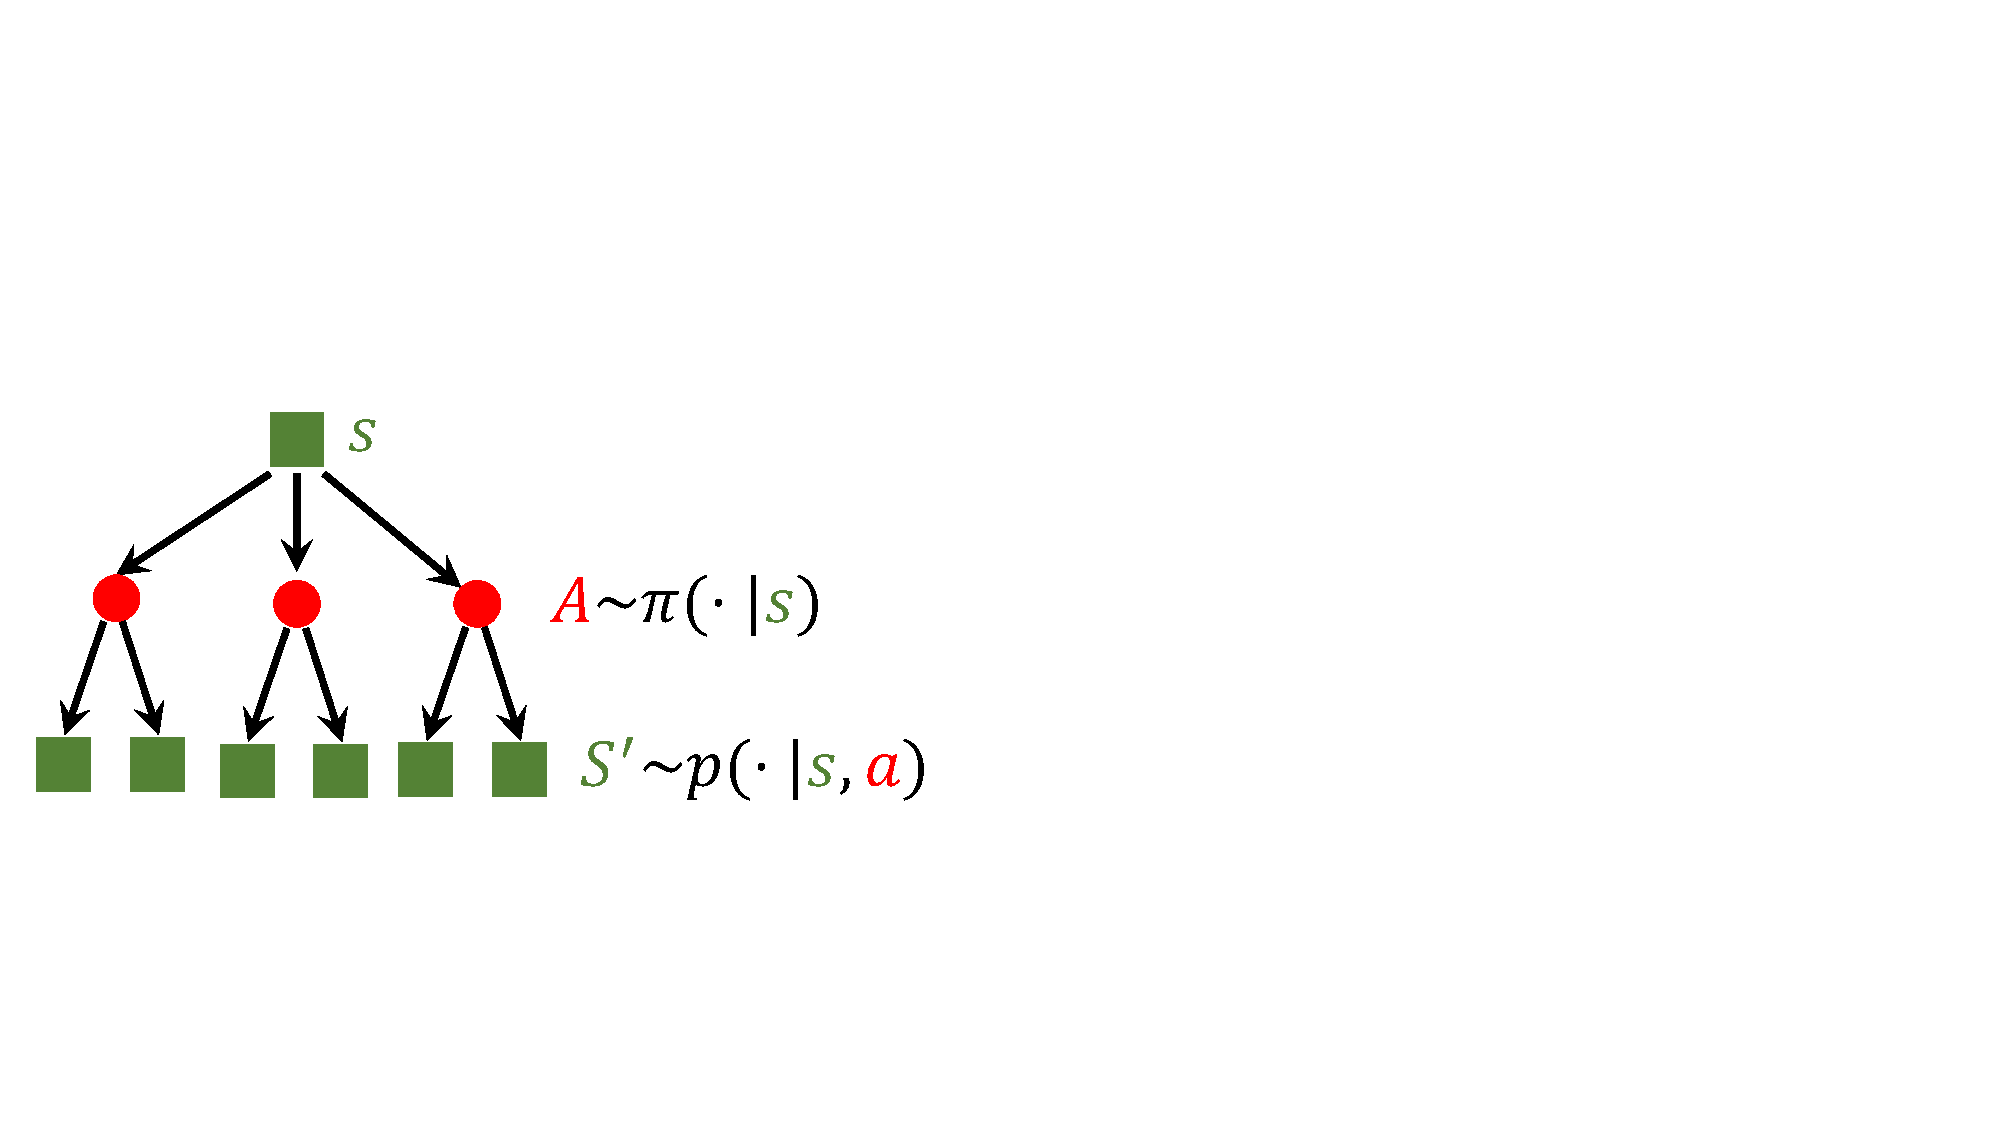
\includegraphics[width=0.5\linewidth]{figures/randomness.pdf}
    \caption{Illustration of the randomness.
    The action $A$ is randomly sampled according to the policy function.
    The new state $S'$ is randomly sampled according to the state-transition function.
    }
    \label{fig:random}
\end{figure}




\paragraph{Return ($U$):}
Return (aka cumulative future reward) is defined as 
\begin{equation*}
    U_t = R_t + R_{t+1} + R_{t+2} + R_{t+3} + \cdots 
\end{equation*}
Discounted return (aka cumulative discounted future reward) is defined as 
\begin{equation*}
    U_t = R_t + \gamma \cdot R_{t+1} + \gamma^2 \cdot  R_{t+2} + \gamma^3 \cdot  R_{t+3} + \cdots 
\end{equation*}
Here, $\gamma \in (0, 1)$ is the discount rate.
The return $U_t$ is random because the future rewards $R_t, R_{t+1}, R_{t+2}, \cdots $ are unobserved random variables.
Recall that the randomness in the $R_i$ ($i \geq t$) comes from the future states $S_i$ and action $A_{i} $.



\paragraph{Action-value function ($Q_{\pi}$):}
Action-value function $Q_{\pi} (s_t, a_t)$ measures given state $s_t$ and policy $\pi$, how good the action $a_t$ is.
Formally speaking, 
\begin{equation*}
    Q_{\pi} (s_t, a_t)
    \: = \: \EB \big[ U_t \, \big| \, S_t = s_t , A_t = a_t  \big] .
\end{equation*}
The expectation is taken w.r.t.\ the future actions $A_{t+1}, A_{t+2}, \cdots $ and future states $S_{t+1}, S_{t+2}, \cdots $ which are random variables.
Note that $Q_{\pi} (s_t, a_t)$ depends on the policy function $\pi$ and the state-transition function $p$.


\paragraph{Optimal action-value function ($Q^\star $):}
The optimal action-value function $Q^\star (s_t, a_t)$ measures how good the action $a_t$ is at state $s_t$.
Formally speaking, 
\begin{equation*}
    Q^\star (s, a)
    \: = \: \max_{\pi } Q_{\pi} (s, a).
\end{equation*}
Note that $Q^\star (s, a)$ is independent of the the policy function $\pi$.



\paragraph{State-value function ($V_{\pi} $):}
State-value function $V_{\pi} (s_t)$ measures given $\pi$, how good the current situation $s_t$ is.
Formally speaking, 
\begin{equation*}
    V_{\pi} (s_t )
    \: = \: \EB_{A\sim \pi (\cdot | s_t )} \big[ Q_{\pi} (s_t, A)  \big] 
    \: = \: \int_{\AM } \pi (a | s_t ) \cdot Q_{\pi} (s_t, a) \: d \, a .
\end{equation*}
Here, the action $A$ is treated as a random variable and integrated out.




\paragraph{Optimal state-value function ($V^\star $):}
The optimal state-value function $V^\star (s_t)$ measures how good the current situation $s_t$ is.
Formally speaking, 
\begin{equation*}
    V^\star (s )
    \: = \: \max_{\pi } V_{\pi} (s).
\end{equation*}
Note that $V^\star (s)$ is independent of the the policy function $\pi$.



\section{Value-Based Deep Reinforcement Learning}


The optimal action-value function $Q^\star  (s, a)$ can be used to control the agent: observing state $s_t$, the agent performs 
\begin{equation*}
    a_t  \: = \:  \argmax_{a \in \AM } Q^\star (s_t , a ) .
\end{equation*}
The optimal action-value function can be approximated by the neural network $Q (s, a; \w )$ where $\w$ captures the model parameters.
The neural network is called \textbf{Deep Q Network (DQN)}.

There are different designs of network architecture.
Here, we consider the game Super Mario, in which the the action space is discrete: $\AM = \{ \textrm{``left''} , \textrm{``right''}, \textrm{``up''}\}$.
DQN takes state $s_t$ (which can be a screenshot or several most recent screenshots) as input.
The architecture can be 
\begin{equation*}
    \texttt{State} 
    \: \Rightarrow \: 
    \texttt{Conv}
    \: \Rightarrow \: 
    \texttt{Flatten}
    \: \Rightarrow \: 
    \texttt{Dense} 
    \: \Rightarrow \: 
    \texttt{Values} .
\end{equation*}
In the Super Mario example, DQN outputs a 3-dimensional vector, e.g., $ [200, 100, 250]$, whose entries corresponds to the three actions.
Then the action should be 
\begin{equation*}
    a_t \: = \: \argmax_{a} Q (s_t , a ; \w ).
\end{equation*}
Since $Q (s_t , \textrm{``up''} ; \w ) = 250$ is the biggest value among the three,
$a_t=$``up'' will be the selected action.



DQN is typically trained using \textbf{temporal different (TD) learning} \cite{sutton2008convergent,sutton2009fast} which allows for updating the model parameters every time a reward $R_t=r_t$ is observed.
By definition, $U_t = \sum_{i=1} \gamma^{i-t} \cdot R_i$.
Thus 
\begin{equation*}
    U_{t} \: = \: R_t + \gamma \cdot U_{t+1}.
\end{equation*}
TD learning makes use of the fact:
\begin{equation*}
    Q_\pi (s_t, a_t)
    \: = \:
    \EB \big[U_{t} \, \big| \, s_t , a_t \big] 
    \: = \: \EB \big[ R_t + \gamma \cdot U_{t+1} \, \big| \, s_t , a_t \big]
    \: = \: \EB \big[ R_t + \gamma \cdot Q_\pi (S_{t+1}, A_{t+1}) \, \big| \, s_t , a_t \big].
\end{equation*}
Since $Q (s_t, a_t; \w) \approx \max_{\pi} \EB [U_t | s_t, a_t]$, we have
\begin{equation*}
    Q (s_t, a_t; \w)  \: \approx \:  r_t + \gamma \cdot Q (s_{t+1}, a_{t+1}; \w) . 
\end{equation*}
Before observing $R_t$, the expected return was
\[
q_t \: = \: Q(s_t , a_t; \w)
\]
After observing $R_t=r_t$, the expected return is updated to
\[
y_t \: = \: r_t + \gamma \cdot Q(s_{t+1} , a_{t+1}; \w),
\]
which is called \textbf{TD target}.
The \textbf{TD error} is $\delta_t = q_t - y_t$.
We seek to encourage a small TD error and thus define the loss:
\begin{equation*}
    L_t \: = \: \frac{1}{2} \delta_t^2 \: = \: \frac{1}{2} \big[ Q (s_t , a_t ; \w ) - y_t \big]^2 .
\end{equation*}
Pretend $y_t$ is not a function of $\w$.
Then the gradient is
\begin{equation*}
    \g_t
    \: \triangleq \: \frac{\partial \, L_t }{\partial \, \w } \Big|_{\w=\w_t }
    \: = \: \delta_t \cdot \frac{\partial \, Q (s_t , a_t ; \w ) }{\partial \, \w } \Big|_{\w=\w_t } .
\end{equation*}
The DQN can be updated by performing a gradient descent: $\w_{k+1} \longleftarrow \w_{k} - \alpha \cdot \g_t $ where $\alpha$ is the learning rate.


\section{Policy-Based Deep Reinforcement Learning} \label{sec:policy}



The policy function $\pi  (a | s)$ can be used to control the agent: observing the state $S_t = s_t$, the agent randomly samples an action: 
\begin{equation*}
    a_t  \: \sim \:  \pi (\cdot | s_t ) .
\end{equation*}
The policy function can be approximated by the neural network $\pi (a | s; \tha )$ where $\tha$ captures the model parameters.
The neural network is called \textbf{policy network}.




There are different designs of network architecture.
Here, we also consider the game Super Mario, in which the the action space is discrete: $\AM = \{ \textrm{``left''} , \textrm{``right''}, \textrm{``up''}\}$.
The policy network takes observed state s (which can be a screenshot) as input.
The architecture can be 
\begin{equation*}
    \texttt{State} 
    \: \Rightarrow \: 
    \texttt{Conv}
    \: \Rightarrow \: 
    \texttt{Flatten}
    \: \Rightarrow \: 
    \texttt{Dense} 
    \: \Rightarrow \: 
    \texttt{Softmax}
    \: \Rightarrow \: 
    \texttt{Probabilities} .
\end{equation*}
In the Super Mario example, DQN outputs a 3-dimensional vector, e.g., $\pp = [0.2, 0.1, 0.7]$, whose entries corresponds to the three actions.
Then the action will be randomly sampled:
\begin{equation*}
    \PB \big( A = \textrm{``left''} \big) = 0.2, \qquad
    \PB \big( A = \textrm{``right''} \big) = 0.1, \qquad
    \PB \big( A = \textrm{``up''} \big) = 0.7.
\end{equation*}
All of the three actions may be selected.
If the random sampling is independently repeated 1000 times, then around 200 observations of $A$ are ``left'', around 100 are ``right'', and around 700 are ``up''.




The policy network can be learned using \textbf{policy gradient} algorithms.
If the actions are discrete, then the state-value function can be written as:
\begin{equation} \label{eq:state_value}
    V_\pi (s ) \: = \: \sum_{a \in \AM} \pi (a | s) \cdot Q_\pi  (s, a)  .
\end{equation}
Policy-based learning uses the policy network $\pi (a | s; \tha )$ to approximate the policy function $\pi (a | s)$.
With the approximation of policy function, $V_\pi (s )$ is approximated by
\begin{equation*}
    V (s ; \tha ) \: = \: \sum_{a \in \AM} \pi (a | s; \tha ) \cdot Q_\pi  (s, a)  .
\end{equation*}
Policy gradient is the derivative of $ V (s ; \tha )$ w.r.t.\ $\tha $ \cite{sutton2000policy}:
\begin{eqnarray*}
    \frac{\partial \, V (s ; \tha )}{\partial \, \tha }
    & = & \frac{\partial \, \sum_{a \in \AM} \pi (a | s; \tha ) \cdot Q_\pi  (s, a)  }{\partial \, \tha } \\
    & = & \sum_{a \in \AM} \frac{\partial \,  \pi (a | s; \tha ) \cdot Q_\pi  (s, a)  }{\partial \, \tha } \\
    & = & \sum_{a \in \AM}  Q_\pi  (s, a)  \cdot \frac{\partial \,  \pi (a | s; \tha )  }{\partial \, \tha } \\
    & = & \sum_{a \in \AM}  Q_\pi  (s, a) \cdot \pi (a | s; \tha )  \cdot \frac{\partial \,  \log \pi (a | s; \tha )  }{\partial \, \tha } .
\end{eqnarray*}
Here, the third identity follows from that $Q_\pi  (s, a)$ does not depend on $\tha$;\footnote{This assumption is too strong. Since $Q_\pi$ depends on the policy function $\pi$, $Q_{\pi}$ can depend on $\tha$. Here, the assumption is used to simplify the derivation.}
the last identity follows from that $\frac{\partial \, \log f (x)}{\partial \, x} = \frac{1}{f (x)}\cdot \frac{\partial f(x)}{\partial \, x}$.
The above equation can be equivalently written as
\begin{equation} \label{eqn:policy_grad}
    \frac{\partial \, V (s ; \tha )}{\partial \, \tha }
    \: = \: \EB_{A \sim \pi (\cdot | s , \theta )} \bigg[  Q_\pi  (s, a)  \cdot \frac{\partial \,  \log \pi (A | s; \tha )  }{\partial \, \tha }  \bigg] .
\end{equation}
Recall that the approximate state-value function $V (s ; \tha )$ indicates how good the situation $s$ is if policy $\pi (a | s; \tha )$ is used.
We thereby have the motivation to update $\tha$ so that $V (s ; \tha )$ will increase (which means the situation is better.)
Thus, the policy network can be updated by policy gradient ascent:
\begin{equation*}
    \tha_{t+1} \: \longleftarrow \: \tha_t + \beta \cdot \frac{\partial \, V (s ; \tha )}{\partial \, \tha } \bigg|_{\theta = \theta_{t}} ,
\end{equation*}
where $\beta$ is the learning rate.

\begin{remark}
The derivation of policy gradient written in the above is not rigorous!
It is a simplified version to make the policy gradient easy to understand.
To be rigorous, we must take into account that $Q_\pi$ depends on the policy $\pi$ and is thereby a function of $\tha$.
However, even is $Q_\pi$'s dependence on $\tha$ is taken into account, the resulting policy gradient is the same to \eqref{eqn:policy_grad}.
\end{remark}


To this end, we defined the policy network and derived the policy gradient in \eqref{eqn:policy_grad}.
However, there are two unsolved problems.
First, the expectation in \eqref{eqn:policy_grad} maybe intractable; this is typically the case when the action space $\AM$ is continuous, e.g., $\AM=[0, 1]$.
Second, the action-value $Q_\pi  (s, a) $ is unknown.
We answer the two questions one by one.


\textbf{What if the expectation in \eqref{eqn:policy_grad} is intractable?}
If the action space $\AM$ is continuous, then the expectation (which is an integration) is typically intractable.
Given state $S_t=s_t$, if the action $A_t = a_t$ is randomly sampled according to the PDF $\pi (\cdot | s_t ; \tha )$, then 
\begin{equation*}
    \tilde{\g}_t
    \: = \: Q_\pi  (s_t, a_t)  \cdot \frac{\partial \,  \log \pi (a_t | s_t; \tha )}{\partial \, \tha }
\end{equation*}
is an unbiased estimate of $\frac{\partial \, V (s_t ; \mathbf{\theta} )}{\partial \,\mathbf{ \theta} }$.
We can think of $\g_{\theta } (\tha )$ as a stochastic gradient and update $\tha$ using stochastic gradient ascent.


\textbf{How do we know the action-value $Q_\pi  (s, a) $?}
There can be two solutions: first, use the observed return $r_t$ instead of $Q_\pi  (s, a) $; second, approximate $Q_\pi  (s, a) $ using a neural network.
The two solutions are described in the following:
\begin{itemize}
\item
    Play a game to the end, obtain all the rewards $r_1, r_2, \cdots , r_T$, and compute the returns $u_1, u_2, \cdots , u_T$ using the equation $u_t = \sum_{i=t}^T \gamma^{i-t} \cdot r_i$.
    Since $Q_\pi  (s_t, a_t) = \EB [U_t | s_t, a_t , \pi ]$, we can use $u_t$ to replace $Q_\pi  (s_t, a_t) $.
    In this way, the policy gradient \eqref{eqn:policy_grad} at time step $t$ becomes
    \begin{equation*}
        \frac{\partial \, V (s_t ; \tha )}{\partial \, \tha }
        \: = \: \EB_{A \sim \pi (\cdot | s_t , \mathbf{\theta} )} \bigg[  u_t  \cdot \frac{\partial \,  \log \pi (A | s_t; \tha )  }{\partial \, \tha }  \bigg] .
    \end{equation*}
    AlphaGo \cite{silver2016mastering} uses this approach.
\item
    Use a value network to approximate $Q_\pi  (s, a) $.
    The value network provides supervision to the policy network.
    The value network can be learned by temporal difference (TD).
    This leads to the actor-critic method which is elaborated on in Section~\ref{sec:actor_critic_rand}.
\end{itemize}




\section{Actor-Critic Methods}  \label{sec:actor_critic}

Section~\ref{sec:actor_critic_rand} follows Section~\ref{sec:policy} and derive the standard (random) actor-critic method.
This approach is suitable for problems with discrete action space.\footnote{For example, Super Mario's action space $\{\textrm{``left''}, \textrm{``right''}, \textrm{``up''} \}$ is a discrete set.}
Section~\ref{sec:actor_critic_det} studies deterministic actor-critic method and learn it using deterministic policy gradient algorithm.
This method is very useful when the actions are continuous.\footnote{For example, a self-driving car's action can be two-dimensional vectors. The first dimension is the steering angle, and the second dimension is acceleration/deceleration. The action space is obviously continuous.}


\subsection{Random Actor-Critic Method} \label{sec:actor_critic_rand}


The actor-critic method has two neural networks.
Policy network $\pi (a | s; \tha ) $, which is called actor, approximates the policy function $\pi (a | s)$.
Value network $q (s, a; \w )$, which is called critic, approximates the action-value function $Q_\pi (a, s)$.
In this way, the state-value function $V_\pi (s )$ is approximated by
\begin{equation*}
    V (s ; \w , \tha )
    \: = \: \EB_{A \sim \pi (\cdot | s; \theta )} \big[ q (s, A ; \w ) \big]
    \: = \: \sum_{a\in \AM} \pi (a | s; \tha ) \cdot  q (s, a ; \w ) .
\end{equation*}
It is not hard to show the policy gradient is
\begin{equation*}
    \frac{\partial \, V (s ; \w , \tha ) }{ \partial \, \tha }
    \: = \: \EB_{A \sim \pi (\cdot | s , \theta )} \bigg[  q  (s, A; \w)  \cdot \frac{\partial \,  \log \pi (A | s; \tha )  }{\partial \, \tha }  \bigg] .
\end{equation*}
The policy network will be updated using (stochastic) policy gradient ascent.
The value network can be updated using temporal different (TD) learning.
The following summarizes one iteration of the algorithm.
\begin{enumerate}
    \item 
    Observe state $s_t$, and then randomly sample action $a_t \sim \pi (\cdot | s_t ; \tha_t )$.
    \item
    Agent performs action $a_t$ and observe reward $r_t$ and new state $s_{t+1}$.
    \item
    Randomly sample action $a_{t+1} \sim \pi (\cdot | s_{t+1} ; \tha_t )$. (Agent does not perform action $a_{t+1}$.)
    \item
    Evaluate the value network and get $q_t = q (s_t , a_t ; \w_t )$ and $q_{t+1} = q (s_{t+1} , a_{t+1} ; \w_t )$.
    \item
    Compute the TD error: $\delta_t = q_t - (r_t + \gamma \cdot q_{t+1})$.
    \item
    Update the value network: $\w_{t+1} \longleftarrow \w_{t} - \alpha \cdot \delta_t \cdot \frac{ \partial \, Q (s_t , a_t ; \w )}{\partial \, \w} \big|_{\w=\w_t }$.
    \item
    Update the policy network: $\tha_{t+1} \longleftarrow \tha_{t} + \beta \cdot q_t \cdot \frac{ \partial \, \log \pi ( a_t | s_t ; \theta )}{\partial \, \theta} \big|_{\theta =\theta_t }$.\footnote{In most papers and books, the update of the policy network is $\tha_{t+1} \longleftarrow \tha_{t} + \beta \cdot \delta_t \cdot \frac{ \partial \, \log \pi ( a_t | s_t ; \theta )}{\partial \, \theta} \big|_{\theta =\theta_t }$.
The difference is that $q_t$ is replaced by $\delta_t$.
Both approaches are correct.
The use of $\delta_t$ is the result of using a baseline which can reduce variance.}
\end{enumerate}
When learning the policy network (actor), the supervision is not from the rewards; instead, the supervision is from the critic's output $q_t = q (s_t , a_t ; \w_t )$.
The actor uses the critic's judgments to improve her performance.
When training the critic, the supervision is from the rewards.
The critic uses ground truth from the environment to make his judgment more accurate.



\subsection{Deterministic Actor-Critic Method}  \label{sec:actor_critic_det}


Throughout, the policy function is defined as the probability density function $\pi (a | s)$, and the action is randomly sampled according to $\pi$.
\textbf{Deterministic policy} is a function that maps state to actions: $\pi: \SM \mapsto \AM$,
where $\SM $ is the state space and $\AM$ is the action space.
Given the state $\s$, the policy function deterministically outputs action $a = \pi (s)$.
Deterministic policy is very useful when the actions are continuous.



Deterministic actor-critic method \cite{silver2014deterministic} has two networks: policy network $\pi (s; \tha )$ and value network $q (s, a ; \w)$; see Figure~\ref{fig:dpg}.
The agent is controlled by the policy network which deterministically maps state $s$ to action $a$.
The value network is used for providing the policy network with supervision.
The two networks can be trained in the following way.

\begin{figure}[!h]
    \centering
    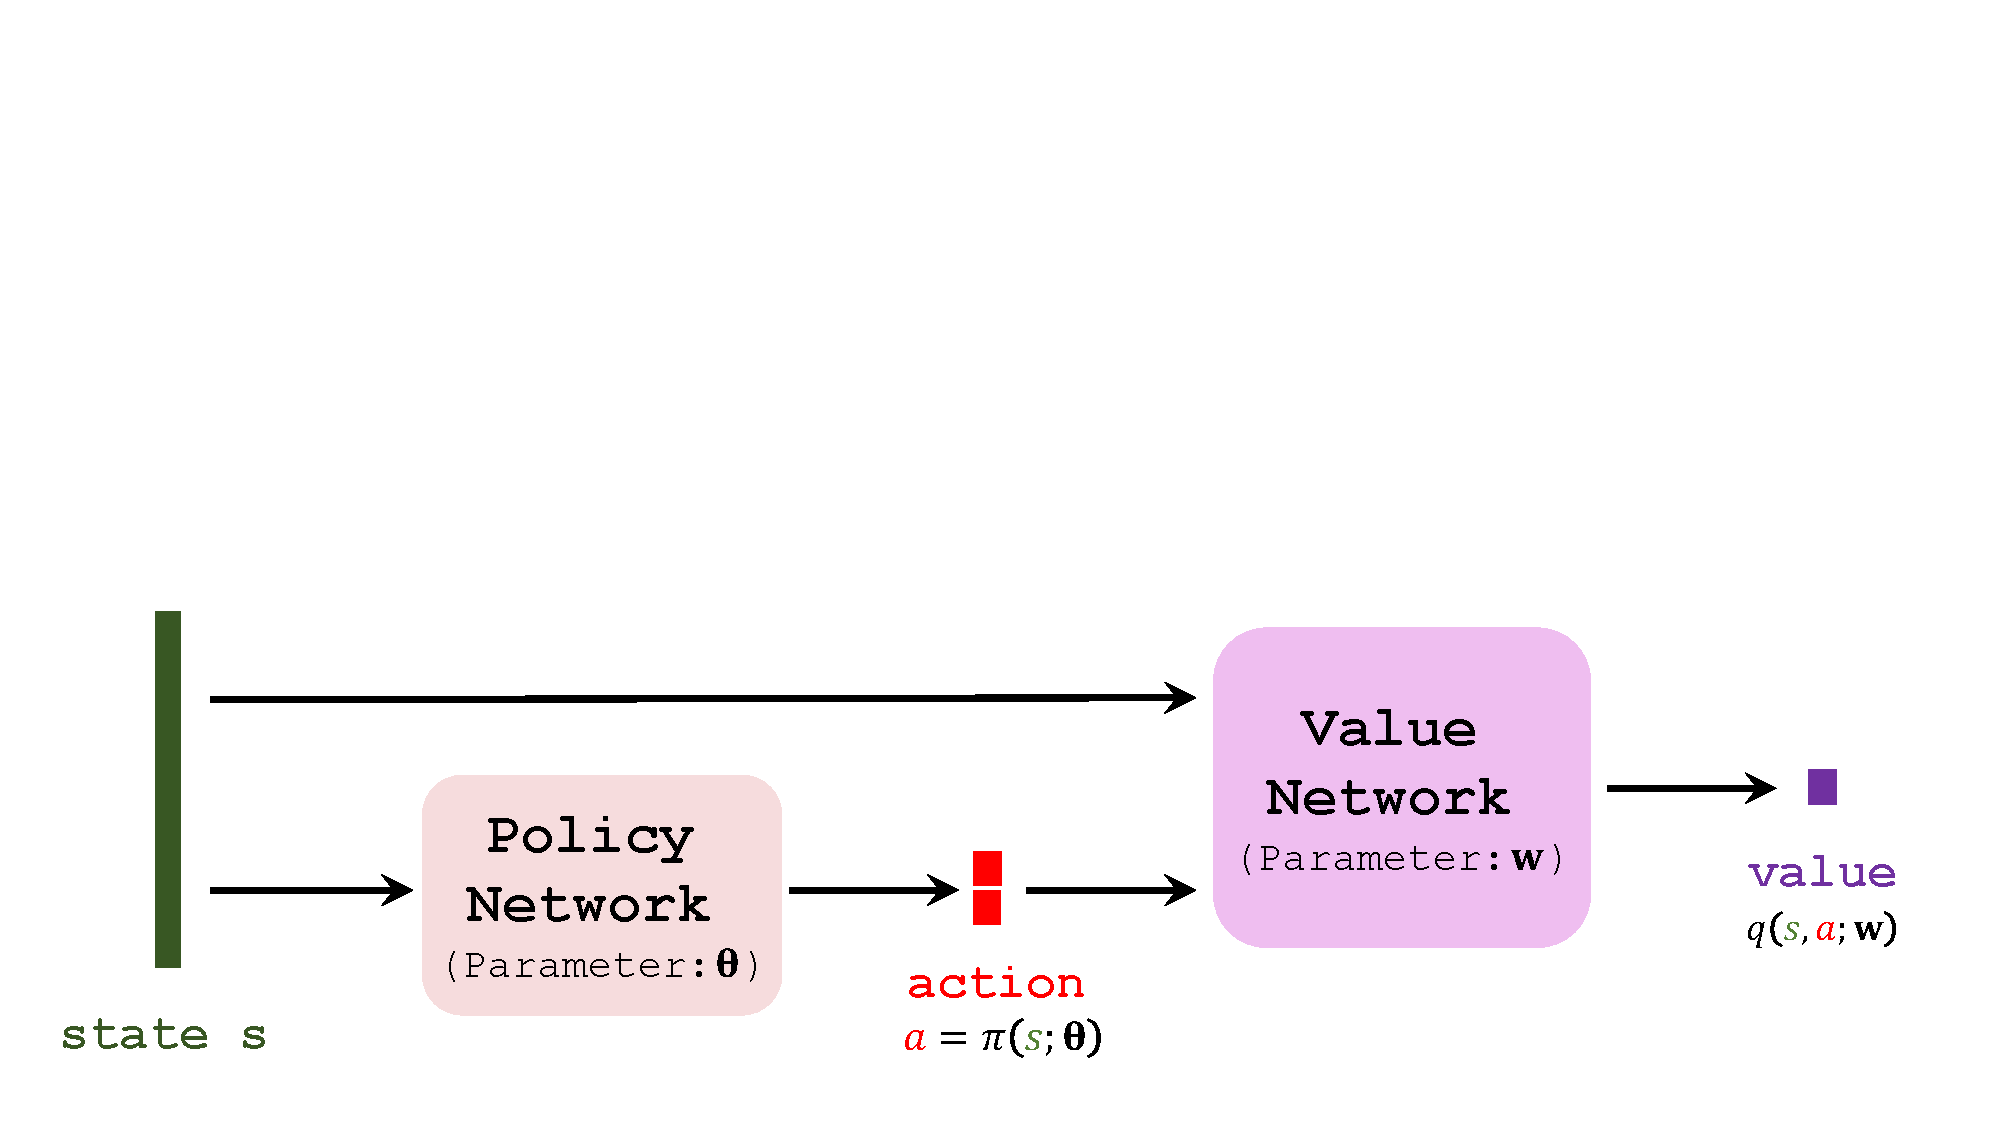
\includegraphics[width=0.8\linewidth]{figures/DPG.pdf}
    \caption{Deterministic actor-critic method.
    The deterministic policy network maps state $s \in \SM$ to action $a \in \AM \subset \RB^2$.
    The two dimensions of $a$ are, for example, the steering angle and acceleration of a self-driving car.
    The value network maps the pair $(s, a)$ to a scalar.
    }
    \label{fig:dpg}
\end{figure}



\paragraph{The value network can be trained by temporal different (TD) learning.}
Let $q_t = q (s_t , a_t ; \w_t )$ be the prediction and $y_t = r_t + \gamma \cdot q (s_{t+1} , a_{t+1} ; \w_t )$ be the TD target.
The TD error is $\delta_t = q_t - y_t$.
The model parameters $\w$ can be updated by $\w_{t+1}\longleftarrow \w_t - \alpha \cdot \delta_t \cdot \frac{\partial \, q (s_t , a_t ; \w )}{\partial \, \w}\big|_{\w=\w_t}$.





\paragraph{Train the policy network by deterministic policy gradient (DPG)} which is totally different from the policy gradient we studied previously.
Note that the value network $q (s_t, a_t; \w)$ evaluates how good it is for the agent to perform action $a_t$ at state $s_t$.
The policy network has motivation to update its parameters $\tha$ so that the action $a_t = \pi (s_t ; \tha)$ will get a higher evaluation.
Intuitively speaking, the policy network (actor) wants to change herself so that the evaluation given by the value network (critic) will increase.
The derivative of the objective, i.e., $q (s_t, a_t; \w)$, w.r.t.\ the policy network's parameters $\tha$ is
\begin{equation*}
    \g (\tha) 
    \: = \: \frac{\partial \, q (s_t , \pi (s_t ; \theta) ; \w )}{\partial \, \theta}
    \: = \: \frac{\partial \, \pi (s_t ; \theta) }{\partial \, \theta} 
    \cdot  \frac{\partial \, q (s_t , a; \w )}{\partial \, a} \bigg|_{a=\pi (s_t ; \theta) } ,
\end{equation*}
where the second identity follows from the chain rule.
The policy network is updated by performing gradient ascent: $\tha_{t+1} \longleftarrow \tha_t + \beta \cdot \g (\tha_t )$.




\bibliographystyle{plainnat}
\bibliography{bib/rl}


\end{document}
